\section{Context} \subsection{}\label{}

\begin{frame}{M2CAI Workflow Dataset}
	
		\begin{figure}
			\centering
			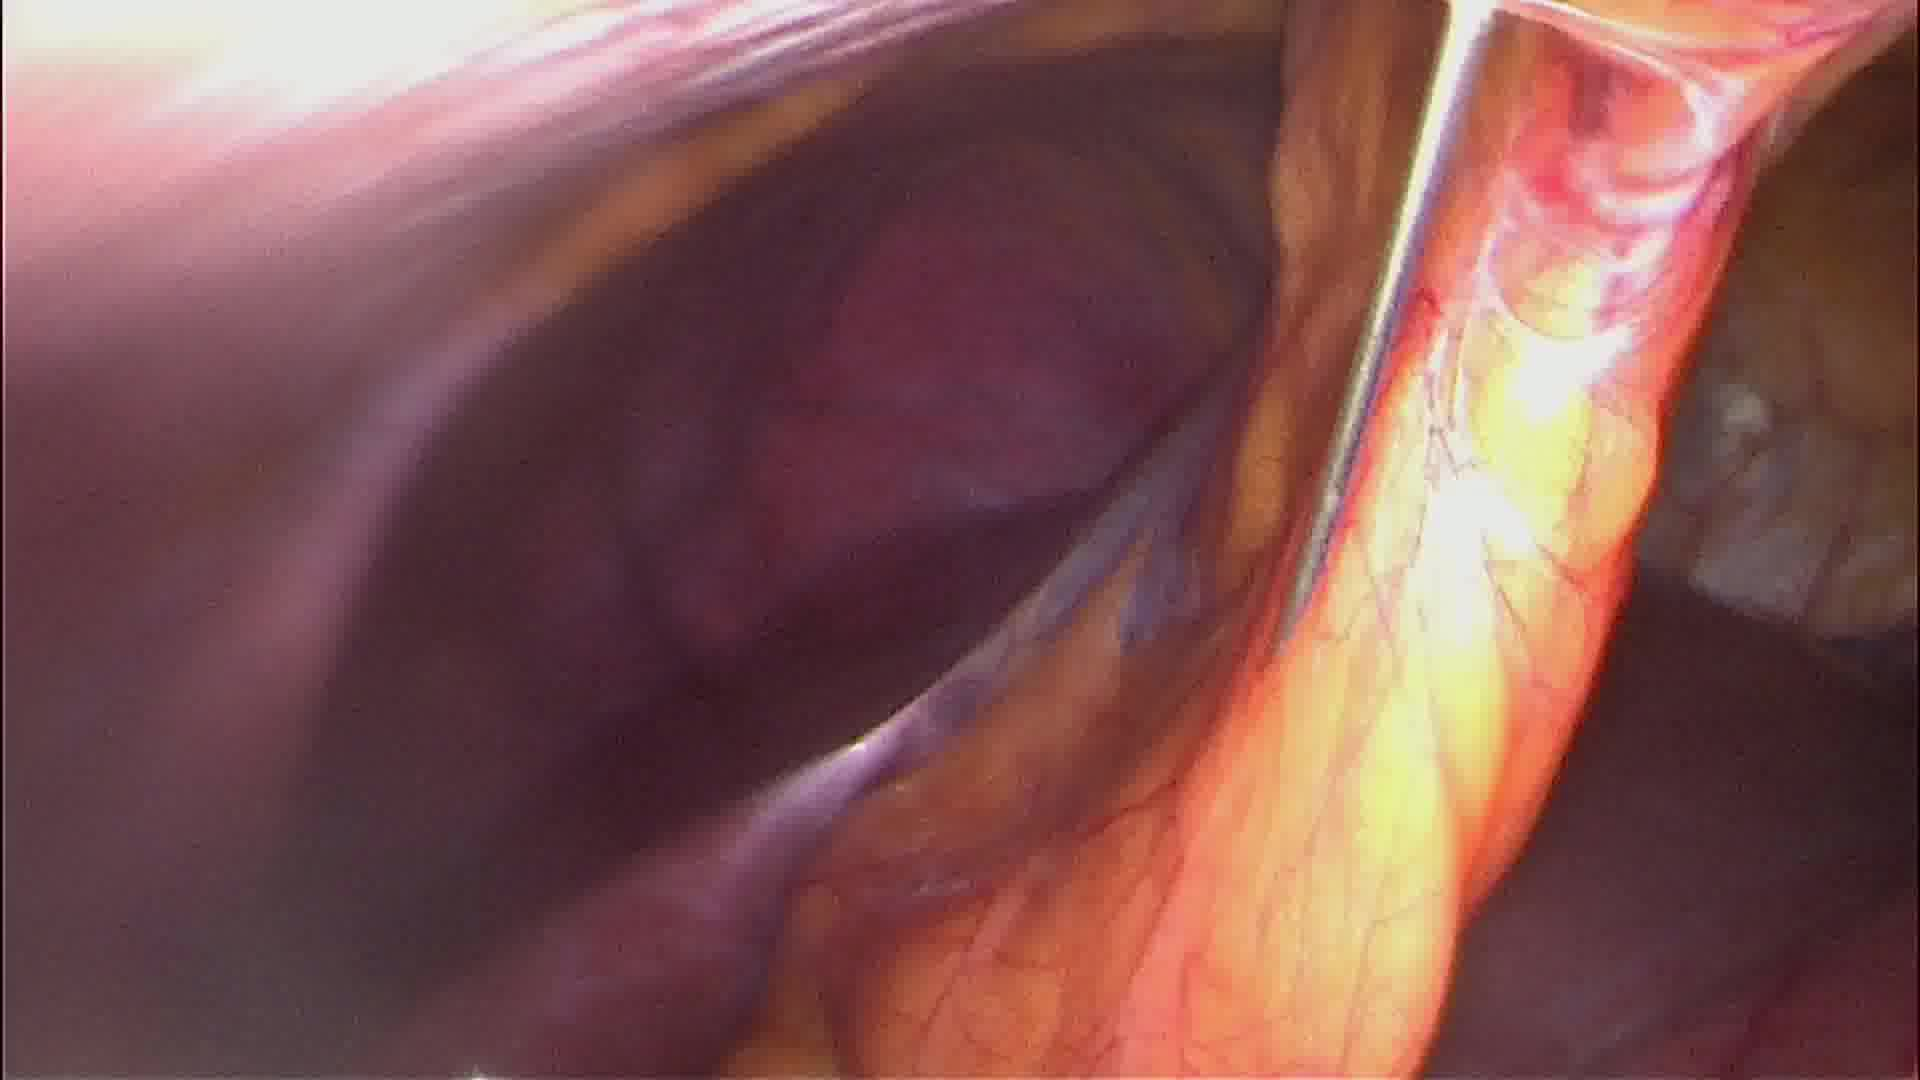
\includegraphics[width=.45\linewidth]{images/m2cai.jpg}
			%		\caption{80000 train images, 20000 test images, 101 classes}
			\label{fig:2images}
		\end{figure}
	
	Videos resolution is 1920 x 1080, shot at 25 frames per second at the IRCAD research center in Strasbourg, France.
	
	\begin{itemize}
		\item 27 training videos ranging from 15mn to 1hour%(67,595 images)
		%\item 22 train videos %(59,493 images)
		%\item 5 val videos %(8,062 images)
		\item 15 test videos %(28,732 images)
		%\item 8 classes (CleaningCoagulation, CalotTriangleDissection, CLippingCutting, etc.)
	\end{itemize}
	
\end{frame}

\begin{frame}{M2CAI Workflow Dataset}

	1 of 8 classes for each frames:
	\begin{itemize}
		\item TrocarPlacement
		\item Preparation
		\item CalotTriangleDissection
       	\item ClippingCutting
       	\item GallbladderDissection
       	\item GallbladderPackaging
       	\item CleaningCoagulation
       	\item GallbladderRetraction
    \end{itemize}

\end{frame}

\begin{frame}{M2CAI Workflow Goal and Measure}
	
	  Online prediction: $P(y | x_i, x_{i-1}, x_{i-2}, ...)$  
		
		$x_i$:= frame $i$, and $y$:= classes
		
		%Detecting at which of the 8 phases of the operation each frames belong.
		
		
		Useful to:
		\begin{itemize}
			\item monitor surgeons
			\item trigger automatic actions
		\end{itemize}
		
		
		Measures:
		- Jaccard similarity coefficient:
	    $J(A,B) = \frac{| A \cap B |}{| A \cup B|} = \frac{| A \cap B |}{| A| + |B| - |A \cap B|}$
	    
	  - Accuracy top1: nb frames well classified / nb total frames
		
\end{frame}




\section{Our approach} \subsection{}\label{}

\begin{frame}{Two fold approach}

	\begin{block}{1. Model to classify frames as images}
	\begin{itemize}
		\item Extract features from pre-trained CNN
		\item CNN From Scratch
		\item Fine tuning pre-trained CNN
	\end{itemize}
	\end{block}
	
	\begin{block}{2. Smoothing predictions of our frames classifier}
	\begin{enumerate}	
		\item Averaging predictions over 15 frames % However, the metric allows a 10 second-margin (not problematic)
		\item Hidden Markov Model as a "denoizer" (HMM)
	\end{enumerate}
	\end{block}
	
\end{frame}


\begin{frame}{1. Creating validation set and extracting images}

	Spliting randomly the full training set of 27 videos
	\begin{itemize}
		\item training set: 22 videos
		\item validation set: 5 videos $\{2,9,10,13,27\}$
	\end{itemize}
	
	\vspace{1cm}	
	
	Extracting one frame every 25 frames (1 frame per second)
	\begin{itemize}
		\item training set: 59,493 images
		\item validation set: 8,062 images
		\item testing set: 28,732 images
	\end{itemize}
	

\end{frame}

\begin{frame}{2. Training a frame classifier}

	\begin{figure}[h]
		\centering
		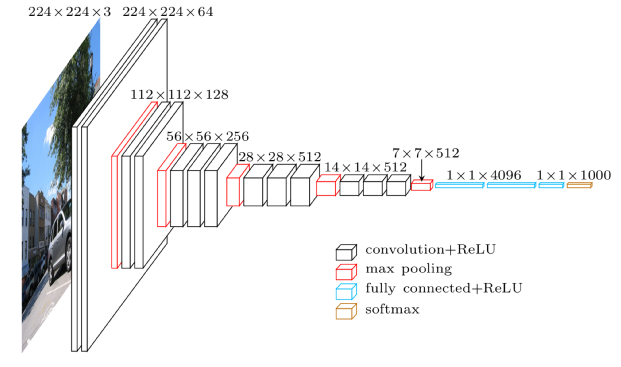
\includegraphics[width=.80\linewidth]{images/vgg16.png}
		\caption{\small Vgg16 \cite{simonyan2014very}, top2 ILSVRC2014}
		\label{fig:quora-invariance-1}
	\end{figure}
	
\end{frame}

\begin{frame}{2. Training a frame classifier}
	
	\begin{block}{\small Pre-trained CNN as Features Extractor}
	\begin{itemize}
		\item Remove last layer, Add new layer output size 8, Train with SGD fixing the pre-trained layers
		\item Extract features somewhere, Train a SVM
	\end{itemize}
	\end{block}
	
	\begin{figure}[h]
		\centering
		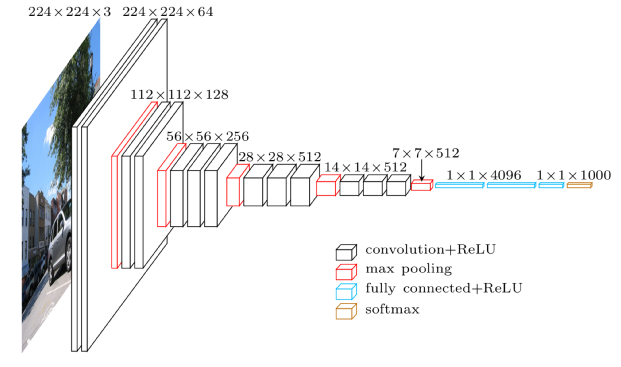
\includegraphics[width=.70\linewidth]{images/vgg16.png}
	\end{figure}

\end{frame}

\begin{frame}{2. Training a frame classifier}

	\begin{block}{\small Training a CNN From Scratch}
	\begin{itemize}
		\item Design specific CNN architecture
		\item Reinitialized architecture designed for large datasets with strong regularization
	\end{itemize}
	\end{block}
	
	\begin{figure}[h]
		\centering
		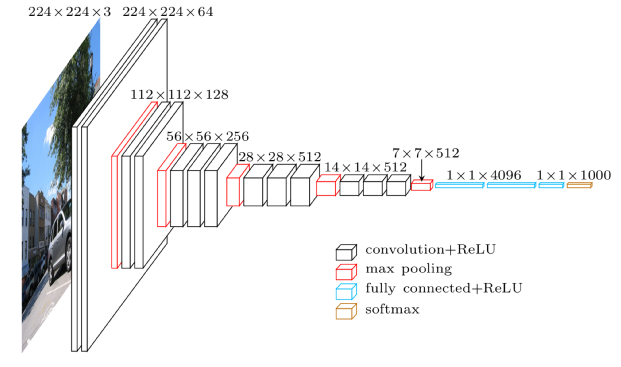
\includegraphics[width=.79\linewidth]{images/vgg16.png}
	\end{figure}
	
\end{frame}


\begin{frame}{2. Training a frame classifier}

	\begin{block}{\small Fine tuning a pre-trained CNN}
	\begin{itemize}
		\item SGD : lr, lrd, ftfactor
		\item Adam : lr, lrd
	\end{itemize}
	\end{block}
	
	\begin{figure}[h]
		\centering
		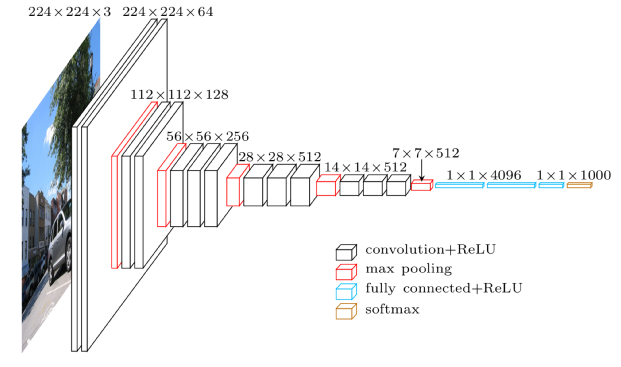
\includegraphics[width=.79\linewidth]{images/vgg16.png}
	\end{figure}

\end{frame}


\begin{frame}{2. Training a frame classifier}

	\begin{table}[h]
		\centering
		\resizebox{300pt}{!}{%
			\begin{tabular}{|c|c|c|c|c|c|}
				\hline
				Model & Input & Param. & Depth & Implem. & Time (ms) \\ \hline \hline
				Vgg16 & 224 & 138M & 16 & GPU &  \\
				InceptionV3 & 399 & 24M & 42 & GPU & \textbf{0} \\
				ResNet-200  & 224 &  & 200 & GPU & \\ \hline
				InceptionV3 & 399 & 24M & 42 & CPU & 0 \\
				\hline
			\end{tabular}}
			\caption{\small Forward+Backward with batches of 30 images.} 
			\label{table:cnnbenchmark}
		\end{table}

\end{frame}


\begin{frame}{3. Smoothing the predictions}

	Averaging the predictions across the last 15 frames (15 seconds)
	
	Hidden Markov Model on the predictions
	3 kind of parameters
	the initial state probabilities
	the matrix of probabilities of transition between states 
	the emissions of observations

\end{frame}

\begin{frame}{3. Smoothing the predictions}

	HMM has 
	
	Training : counting
	
	Offline testing : Viterbi algorithm to obtain the most likely sequence of states
	
	Online testing : to predict $x_t$ we apply Viterbi on the sequence $y_1,...,y_t$

\end{frame}
	
\section{Experiments} \subsection{}\label{}

\begin{frame}{Comparison of frames classifiers}
	
	\begin{table}
	\begin{center}
		\begin{tabular}{|c|c|}
			\hline
			Classification Model & Accuracy (\%) \\
			\hline\hline
			InceptionV3 Extraction & 60.53 \\
			InceptionV3 From Scratch & 69.13 \\
			InceptionV3 Weldon & 78.18 \\
			InceptionV3 Fine-tuned & 79.06 \\
			ResNet200 Fine-tuned & 79.24 \\
			\hline
		\end{tabular}
	\end{center}
	\caption{Accuracy on the validation set.}
	\end{table}

\end{frame}

\begin{frame}{Comparison of temporal smoothing methods}

	\begin{table}
	\begin{center}
		\begin{tabular}{|c|c|c|}
			\hline
			Temporal Method & Accuracy (\%) & Jaccard \\
			\hline\hline
			Avg Smoothing & 85.97 $\pm$ 3.75 & 74.67 $\pm$ 7.87\\
			HMM Online & 88.90 $\pm$ 3.55 & 81.60 $\pm$ 10.49\\
			HMM Offline & 93.47 $\pm$ 3.59 & 87.59 $\pm$ 6.97\\
			\hline
		\end{tabular}
	\end{center}
	\caption{Accuracy Top1 and Jaccard score on the validation set. The variance is computed over all classes.}
	\end{table}

\end{frame}

\begin{frame}{Visualization}

	\begin{figure}
\begin{center}
%\fbox{\rule{0pt}{2in} \rule{0.9\linewidth}{0pt}}
   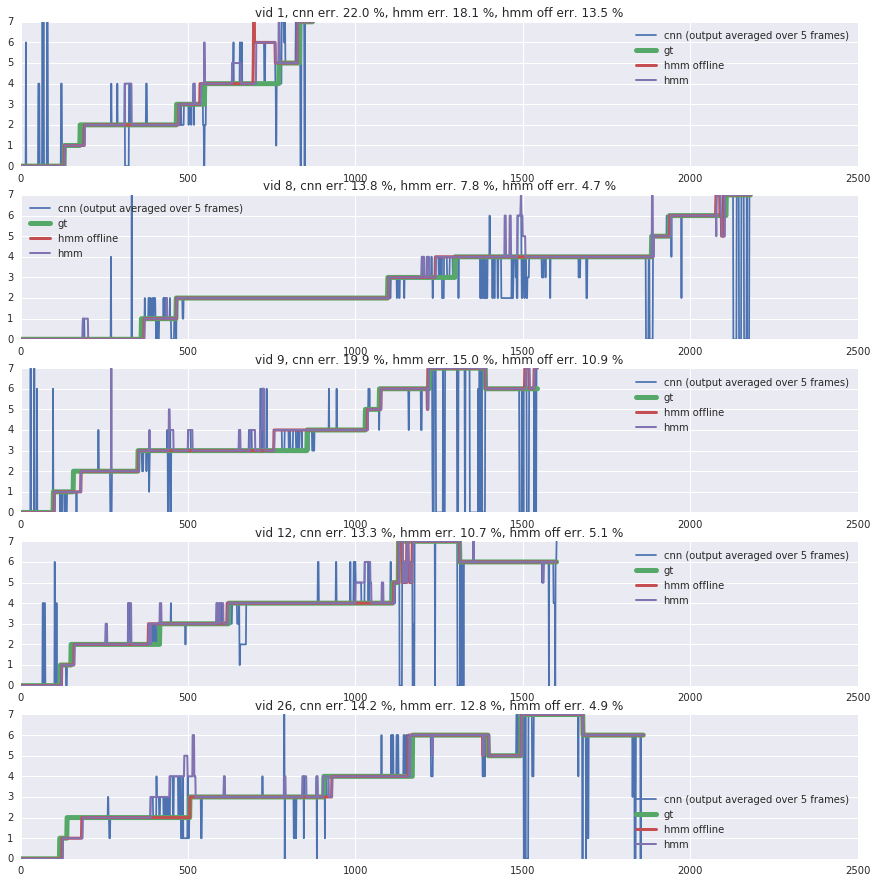
\includegraphics[width=1\linewidth]{../report/images/visu.png}
\end{center}
   \caption{Comparison of our temporal models predictions on the validation set. In blue, our ResNet200 Fine-tuned with average smoothing over 5 frames. In red, the offline predictions of an HMM trained of top of the latter model predictions. In mauve, the online predictions. In green, the ground truth label. }
\label{fig:long}
\label{fig:onecol}
\end{figure}	
	
\end{frame}


\section{Conclusion} \subsection{}\label{}

\begin{frame}{Conclusion}

	\begin{block}{Conclusion}
		\begin{itemize}
			\item Deep Learning efficient %to takle this problem
			\item Fine Tuning most accurate approach %to build a frames classifier
			\item HMM is usefull to smooth the predictions %to add a prior in order to smooth the predictions
		\end{itemize}
	\end{block}
	
	\begin{block}{Future work}
		\begin{itemize}
			\item train on 100\%
			\item ensembling
		\end{itemize}
	\end{block}
	
	Code available: github.com/Cadene/torchnet-m2caiworkflow
	
\end{frame}

\section{References} \subsection{}\label{references}

\begin{frame}[allowframebreaks]{References}
	
	\printbibliography[heading=none]
	
\end{frame}